\section{Latency of big blocks with long tails}

The extended CMS data production and processing tasks that run over
the distributed WLCG infrastructure may occasionally produce corrupted
outputs. That is, one or few files in a datablock which are missing -
resulting from a non-handled failure in the stageout to grid storage -
or have wrong size/checksum.  PhEDEx has been designed to deal with
such data corruption events and is able to detect the corrupted files
- relying on FTS internal checking mechanisms and on pre/post
validation scripts - and tag the corresponding transfers as
failing. Moreover PhEDEx tries to minimize the impact of the corrupted
files on the data placement operations - and in particular on the
transfers throughput - by re-queuing such files with low rank while it
keeps on transferring the rest of the data. As the transfers of the corrupted
files keep on failing systematically, PhEDEx suspends them for a
longer time.

Thus the effect of file corruption during data production is observed,
at data placement level, as a latency tail issue in PhEDEx transfers.
The impact of these missing/corrupt files can only be seen in the last
few percentages of the transfer of the whole block. Hence, while
transfer rates in the first 95\% have higher values, rate in the last
5\% drops off to quite low values as shown in
fig.~\ref{fig:figure-5.1}. In a similar way, $RSkewLast_5$ values (see
eq.~\ref{eq:revskewlast}) are much lower than $Skew_{95}$ values (see
eq.~\ref{eq:skew}) in fig.~\ref{fig:figure-5.2}.

\begin{figure}[htp]
\centering
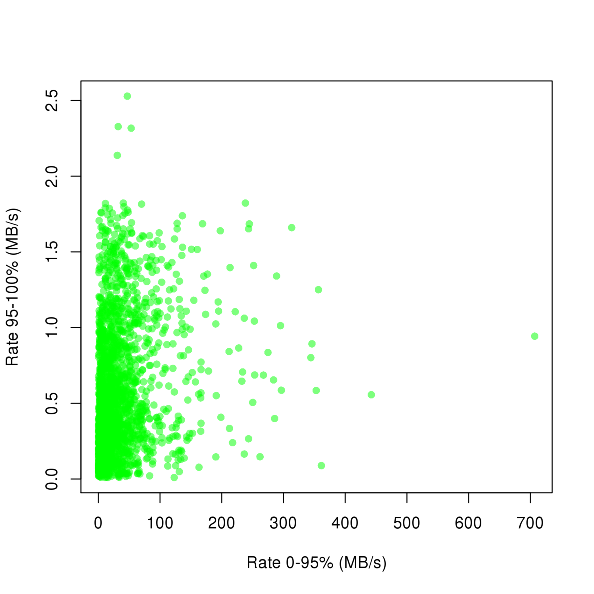
\includegraphics{Figures/figure-51.pdf}
\caption{}\label{fig:figure-5.1}
\end{figure}

\begin{figure}[htp]
\centering
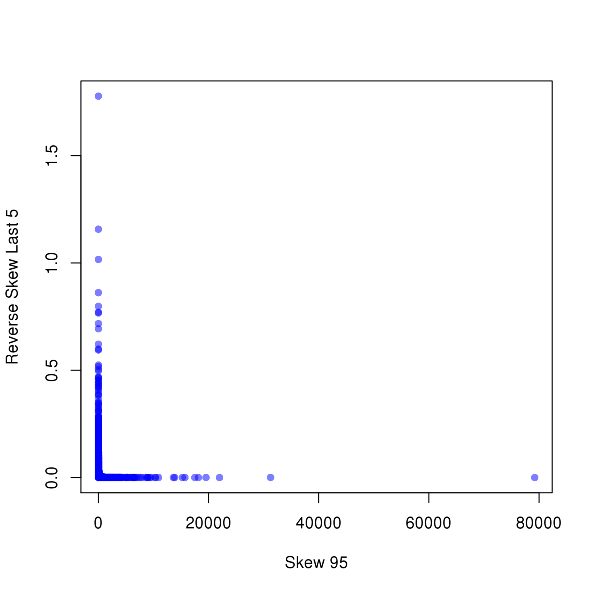
\includegraphics{Figures/figure-52.pdf}
\caption{}\label{fig:figure-5.2}
\end{figure}

The underlying reasons for file production failures have been
extensively investigated by the CMS PhEDEx team.  It was observed that
they are mostly due to transient storage problems, which explains why
only a few files are affected from this issue. Tier-2's grid sites are
particularly exposed to this source of latency as Tier-1's generally
have more reliable storage systems. This can be seen in
fig.~\ref{fig:figure-5.3}.

\begin{figure}[htp]
\centering
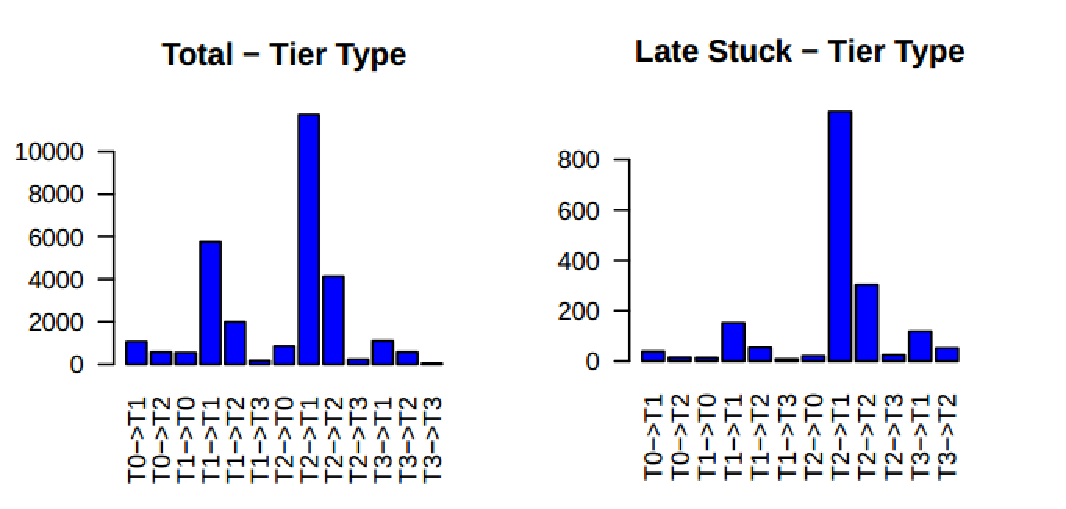
\includegraphics{Figures/figure-53.pdf}
\caption{}\label{fig:figure-5.3}
\end{figure}


Despite only few files for each data sample are concerned, this type
of latency issues can have a very important impact on the CMS
operation. In most cases, in fact, the transferred data is useless to
CMS jobs until a 100\% transfer completion is reached. Thus, it is
quite important to find the “stuck” files being the root cause of the
latency, and fix the identified problems as soon as possible. In most
cases, solving this problem requires a manual expert operator
intervention, consisting of either replacing the file (if it has other
valid replicas) or otherwise invalidating it and announcing it as
lost.
